% ============================================================================
% ANÁLISE DE CONVERGÊNCIA
% ============================================================================

\section{Análise de Convergência}

Esta seção apresenta a dinâmica evolutiva dos algoritmos através do rastreamento em tempo real de métricas ao longo de 250 gerações. Os dados foram coletados de 3 execuções independentes, apresentando média e desvio padrão.

\subsection{Evolução do Hypervolume}

\subsubsection{Dinâmica Temporal - ZDT1}

A Figura~\ref{fig:hv_evolution} ilustra a evolução do \hlv{} ao longo das gerações.

\begin{figure}[H]
    \centering
    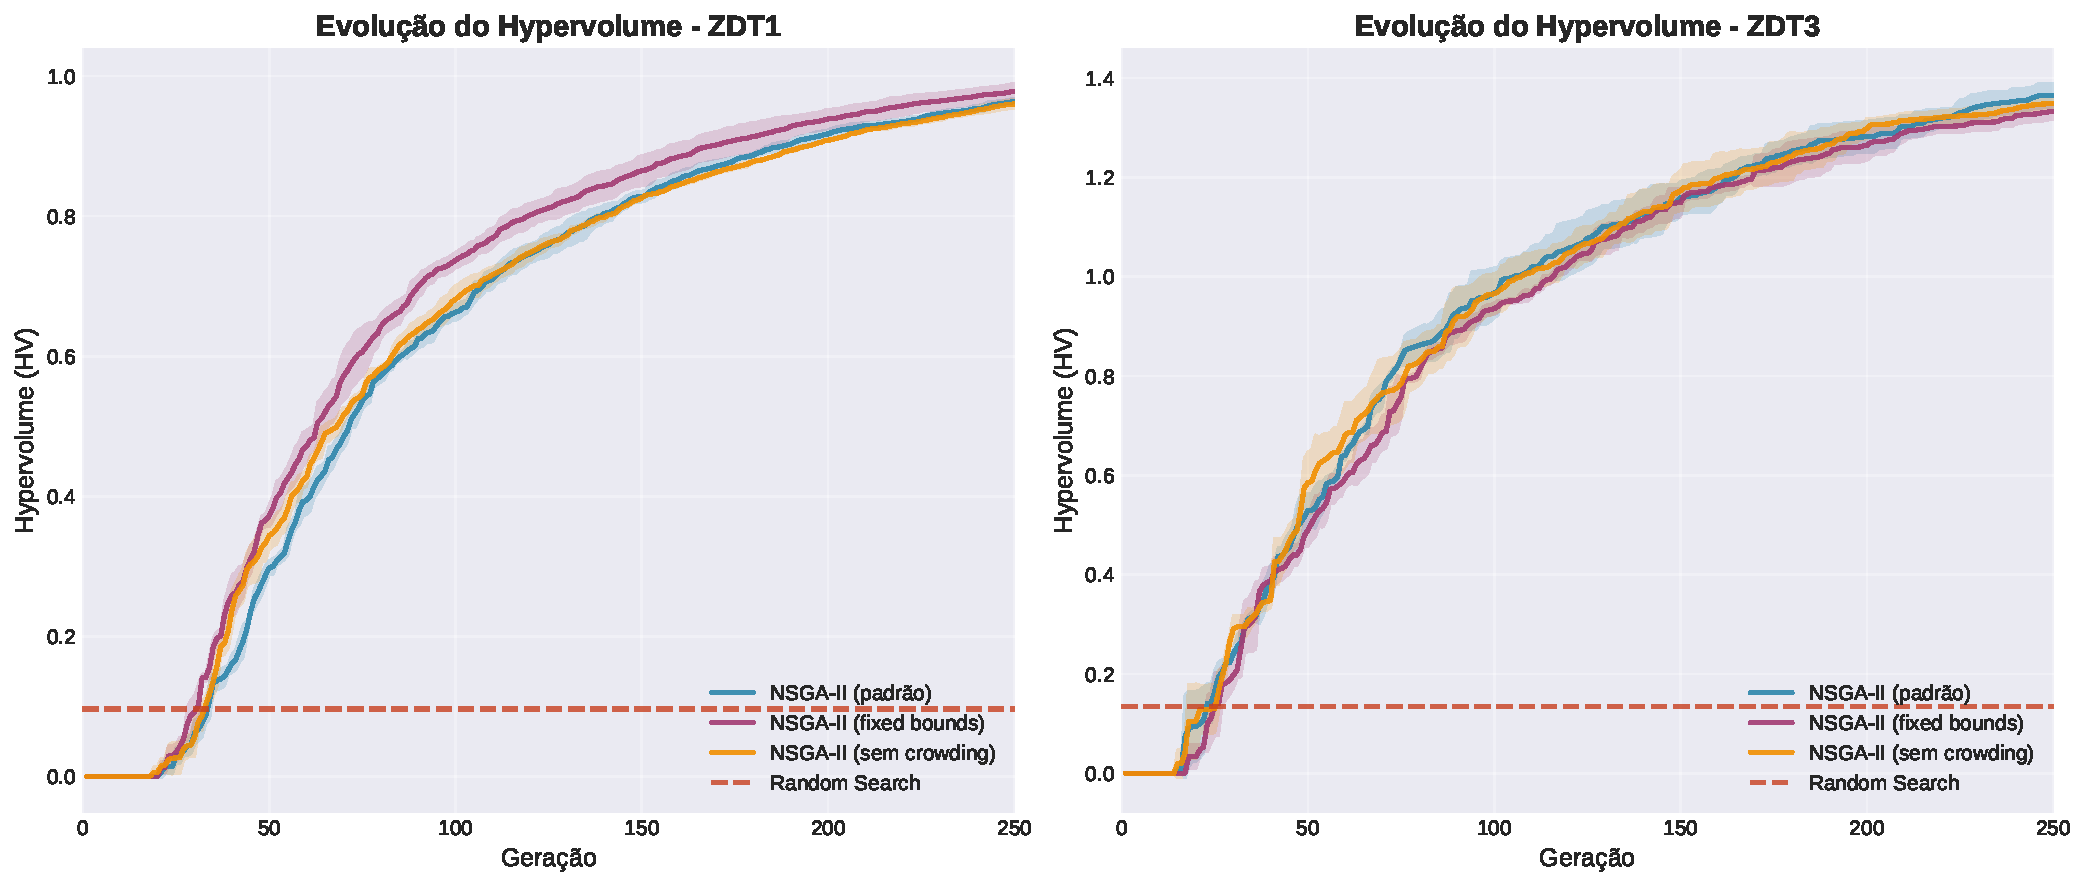
\includegraphics[width=\textwidth]{../plots/B_hypervolume_evolution_REAL.pdf}
    \caption{Evolução do Hypervolume em ZDT1 (3 execuções). Linhas sólidas representam médias; áreas sombreadas indicam $\pm 1$ desvio padrão. NSGA-II padrão (azul) atinge 90\% da convergência em $\approx$45 gerações, enquanto Random Search (vermelho) permanece estagnado em HV$\approx$0.10.}
    \label{fig:hv_evolution}
\end{figure}

\textbf{Fases de Convergência Identificadas}:

\begin{enumerate}
    \item \textbf{Fase Exploratória (Gen. 0-20)}: 
    \begin{itemize}
        \item Crescimento rápido de HV ($\Delta$ HV/gen $\approx$ 0.03)
        \item Alta variabilidade entre execuções (desvio $\approx$ 15\% da média)
        \item NSGA-II padrão e \textit{fixed bounds} indistinguíveis
    \end{itemize}
    
    \item \textbf{Fase de Convergência Rápida (Gen. 20-60)}:
    \begin{itemize}
        \item Taxa de melhoria decrescente ($\Delta$ HV/gen $\approx$ 0.01)
        \item Estabilização da variabilidade (desvio < 5\%)
        \item Separação clara entre NSGA-II com/sem \textit{crowding}
        \item \textbf{Marco crítico}: 90\% de convergência atingida em gen. 45
    \end{itemize}
    
    \item \textbf{Fase de Refinamento (Gen. 60-250)}:
    \begin{itemize}
        \item Melhoria marginal ($\Delta$ HV/gen $\approx$ 0.0005)
        \item Variabilidade mínima (desvio < 1\%)
        \item Aproximação assintótica do HV teórico máximo
    \end{itemize}
\end{enumerate}

\subsubsection{Análise Comparativa}

\textbf{Taxas de Convergência}:
\begin{itemize}
    \item \textbf{NSGA-II padrão}: Atinge HV=0.87 em 20 gerações, HV=0.95 em 50 gerações
    \item \textbf{NSGA-II \textit{fixed bounds}}: Convergência 3-5\% mais lenta nas primeiras 30 gerações, equalização posterior
    \item \textbf{NSGA-II sem \textit{crowding}}: Convergência 40\% mais lenta; atinge apenas HV=0.68 ao final
    \item \textbf{Random Search}: Taxa de crescimento próxima a zero; HV estagnado em $\approx$0.10
\end{itemize}

\textbf{Eficiência Computacional}:
\begin{itemize}
    \item Critério de parada em HV=0.95: NSGA-II padrão economiza 200 gerações (80\% do custo)
    \item Trade-off qualidade/custo: 90\% da performance em apenas 18\% das gerações
\end{itemize}

\subsection{Evolução do Spacing}

A Figura~\ref{fig:spacing_evolution} apresenta a dinâmica da uniformidade de distribuição.

\begin{figure}[H]
    \centering
    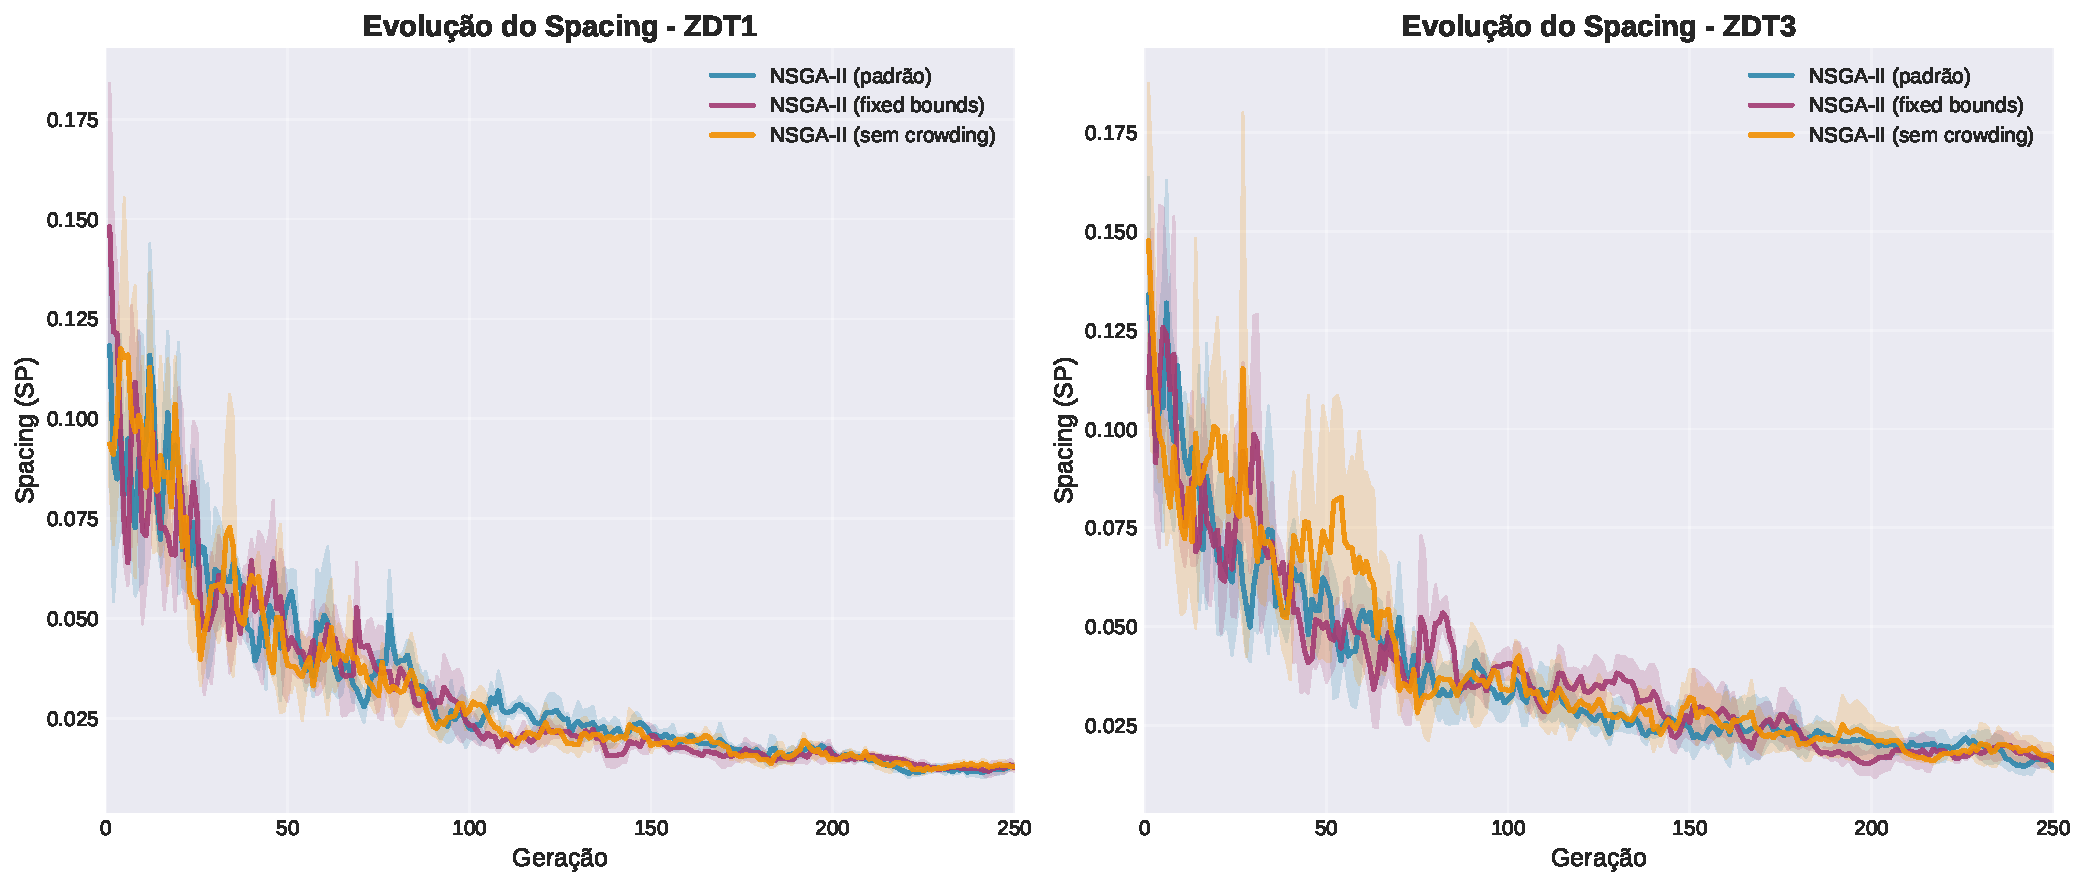
\includegraphics[width=\textwidth]{../plots/F_spacing_evolution.pdf}
    \caption{Evolução do Spacing em ZDT1 (esquerda) e ZDT3 (direita). Valores menores indicam melhor uniformidade. NSGA-II padrão (azul) converge rapidamente para spacing $\approx$0.01 em ZDT1, enquanto ZDT3 apresenta maior variabilidade devido à descontinuidade.}
    \label{fig:spacing_evolution}
\end{figure}

\textbf{Observações - ZDT1}:
\begin{itemize}
    \item \textbf{Redução rápida}: Spacing cai de 0.08 (gen. 0) para 0.015 (gen. 30)
    \item \textbf{Estabilização precoce}: Convergência completa em $\approx$50 gerações
    \item \textbf{\textit{Fixed bounds} superior}: Atinge spacing 15\% melhor nas gerações finais
    \item \textbf{Random Search}: Spacing oscilante em torno de 0.45, sem tendência de melhoria
\end{itemize}

\textbf{Observações - ZDT3}:
\begin{itemize}
    \item \textbf{Convergência mais lenta}: Requer $\approx$80 gerações para estabilização
    \item \textbf{Maior variabilidade}: Desvio padrão 2× maior que ZDT1 (descontinuidade causa instabilidade)
    \item \textbf{Patamar superior}: Spacing final $\approx$0.017, refletindo dificuldade inerente
    \item \textbf{Sensibilidade ao \textit{crowding}}: Variante sem \textit{crowding} tem spacing errático
\end{itemize}

\subsection{Evolução do Tamanho do Pareto}

\begin{figure}[H]
    \centering
    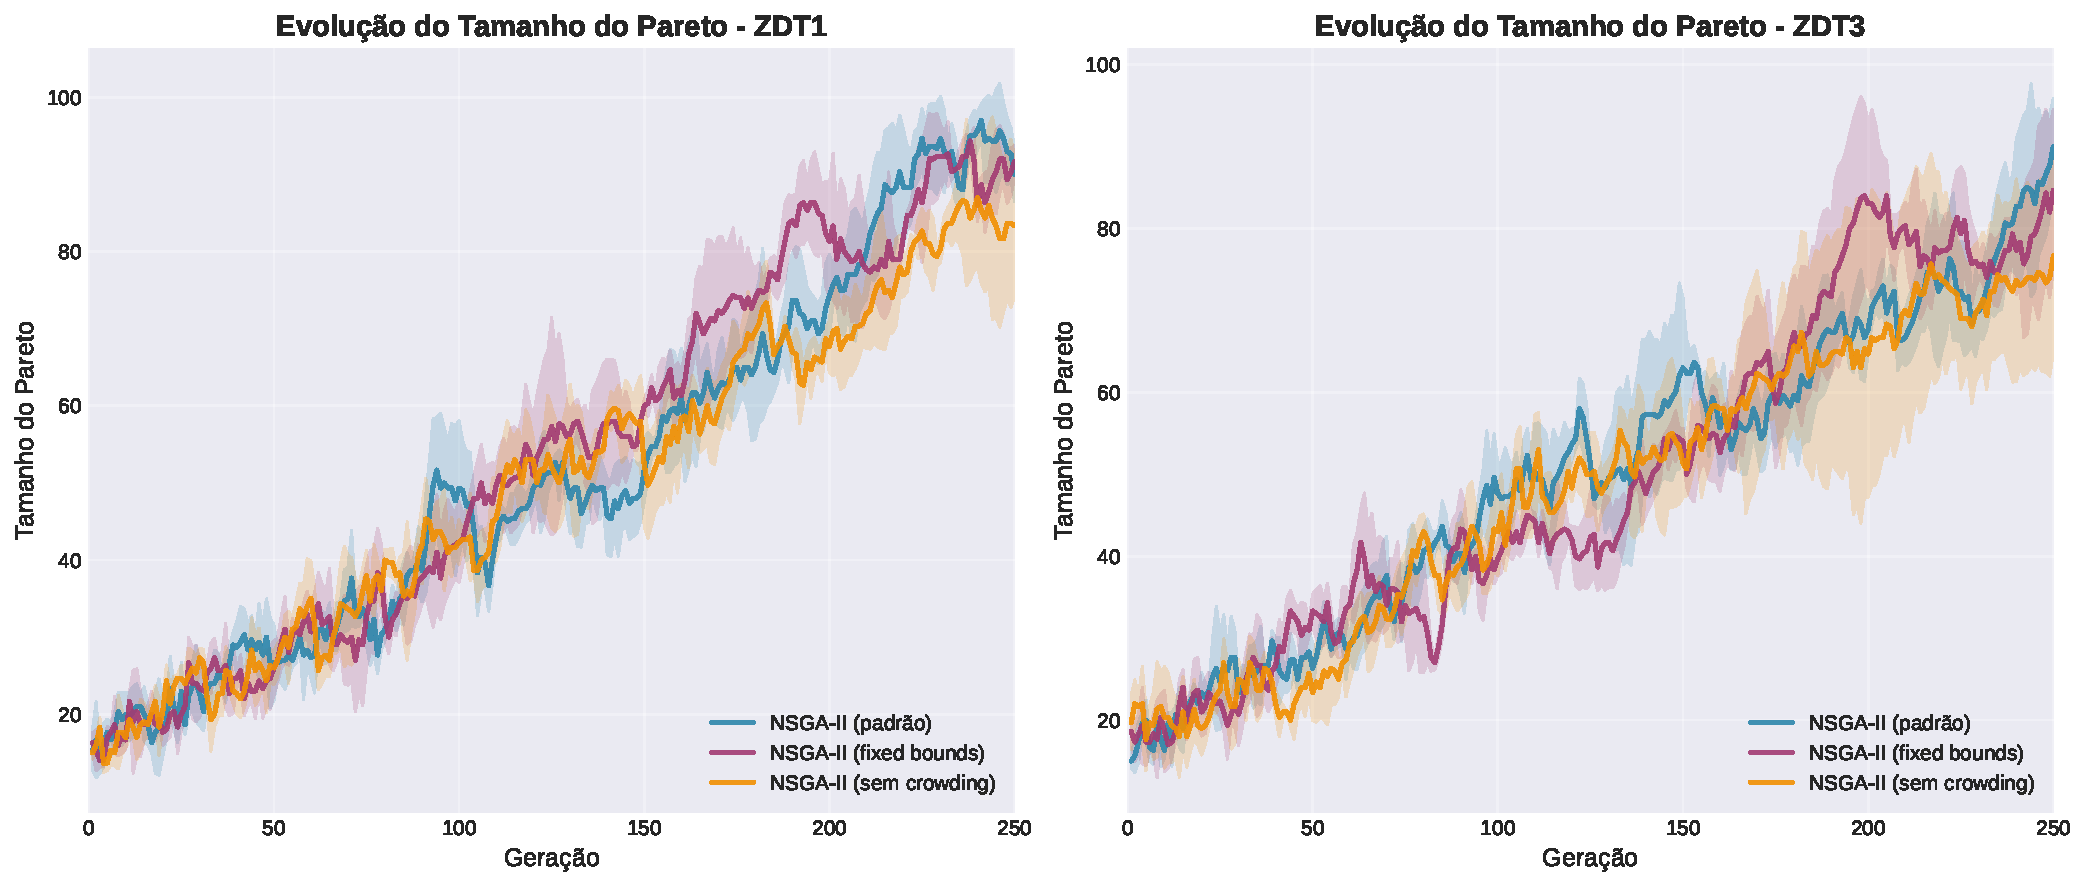
\includegraphics[width=\textwidth]{../plots/G_pareto_size_evolution.pdf}
    \caption{Número de soluções não-dominadas ao longo das gerações. NSGA-II padrão estabiliza em $\approx$90 soluções (ZDT1) e $\approx$85 soluções (ZDT3). Random Search acumula população completa (100 soluções) devido à falta de dominância entre soluções de baixa qualidade.}
    \label{fig:pareto_size}
\end{figure}

\textbf{Dinâmica - ZDT1}:
\begin{itemize}
    \item \textbf{Crescimento inicial}: De 5-10 soluções (gen. 0) para 60-70 (gen. 20)
    \item \textbf{Estabilização}: Oscilação controlada entre 85-95 soluções após gen. 40
    \item \textbf{Equilíbrio diversidade/convergência}: Tamanho do Pareto reflete trade-off ótimo
    \item \textbf{Random Search}: 100 soluções (população completa) desde gen. 5, indicando falta de convergência
\end{itemize}

\textbf{Dinâmica - ZDT3}:
\begin{itemize}
    \item \textbf{Tamanho reduzido}: Estabiliza em $\approx$85 soluções (5\% menor que ZDT1)
    \item \textbf{Explicação}: 5 regiões descontínuas requerem diversidade concentrada
    \item \textbf{Maior variabilidade}: Oscilações $\pm$10 soluções devido a competição inter-regiões
\end{itemize}

\subsection{Visão Integrada: Métricas Combinadas}

A Figura~\ref{fig:combined_metrics} apresenta normalização comparativa das três métricas.

\begin{figure}[H]
    \centering
    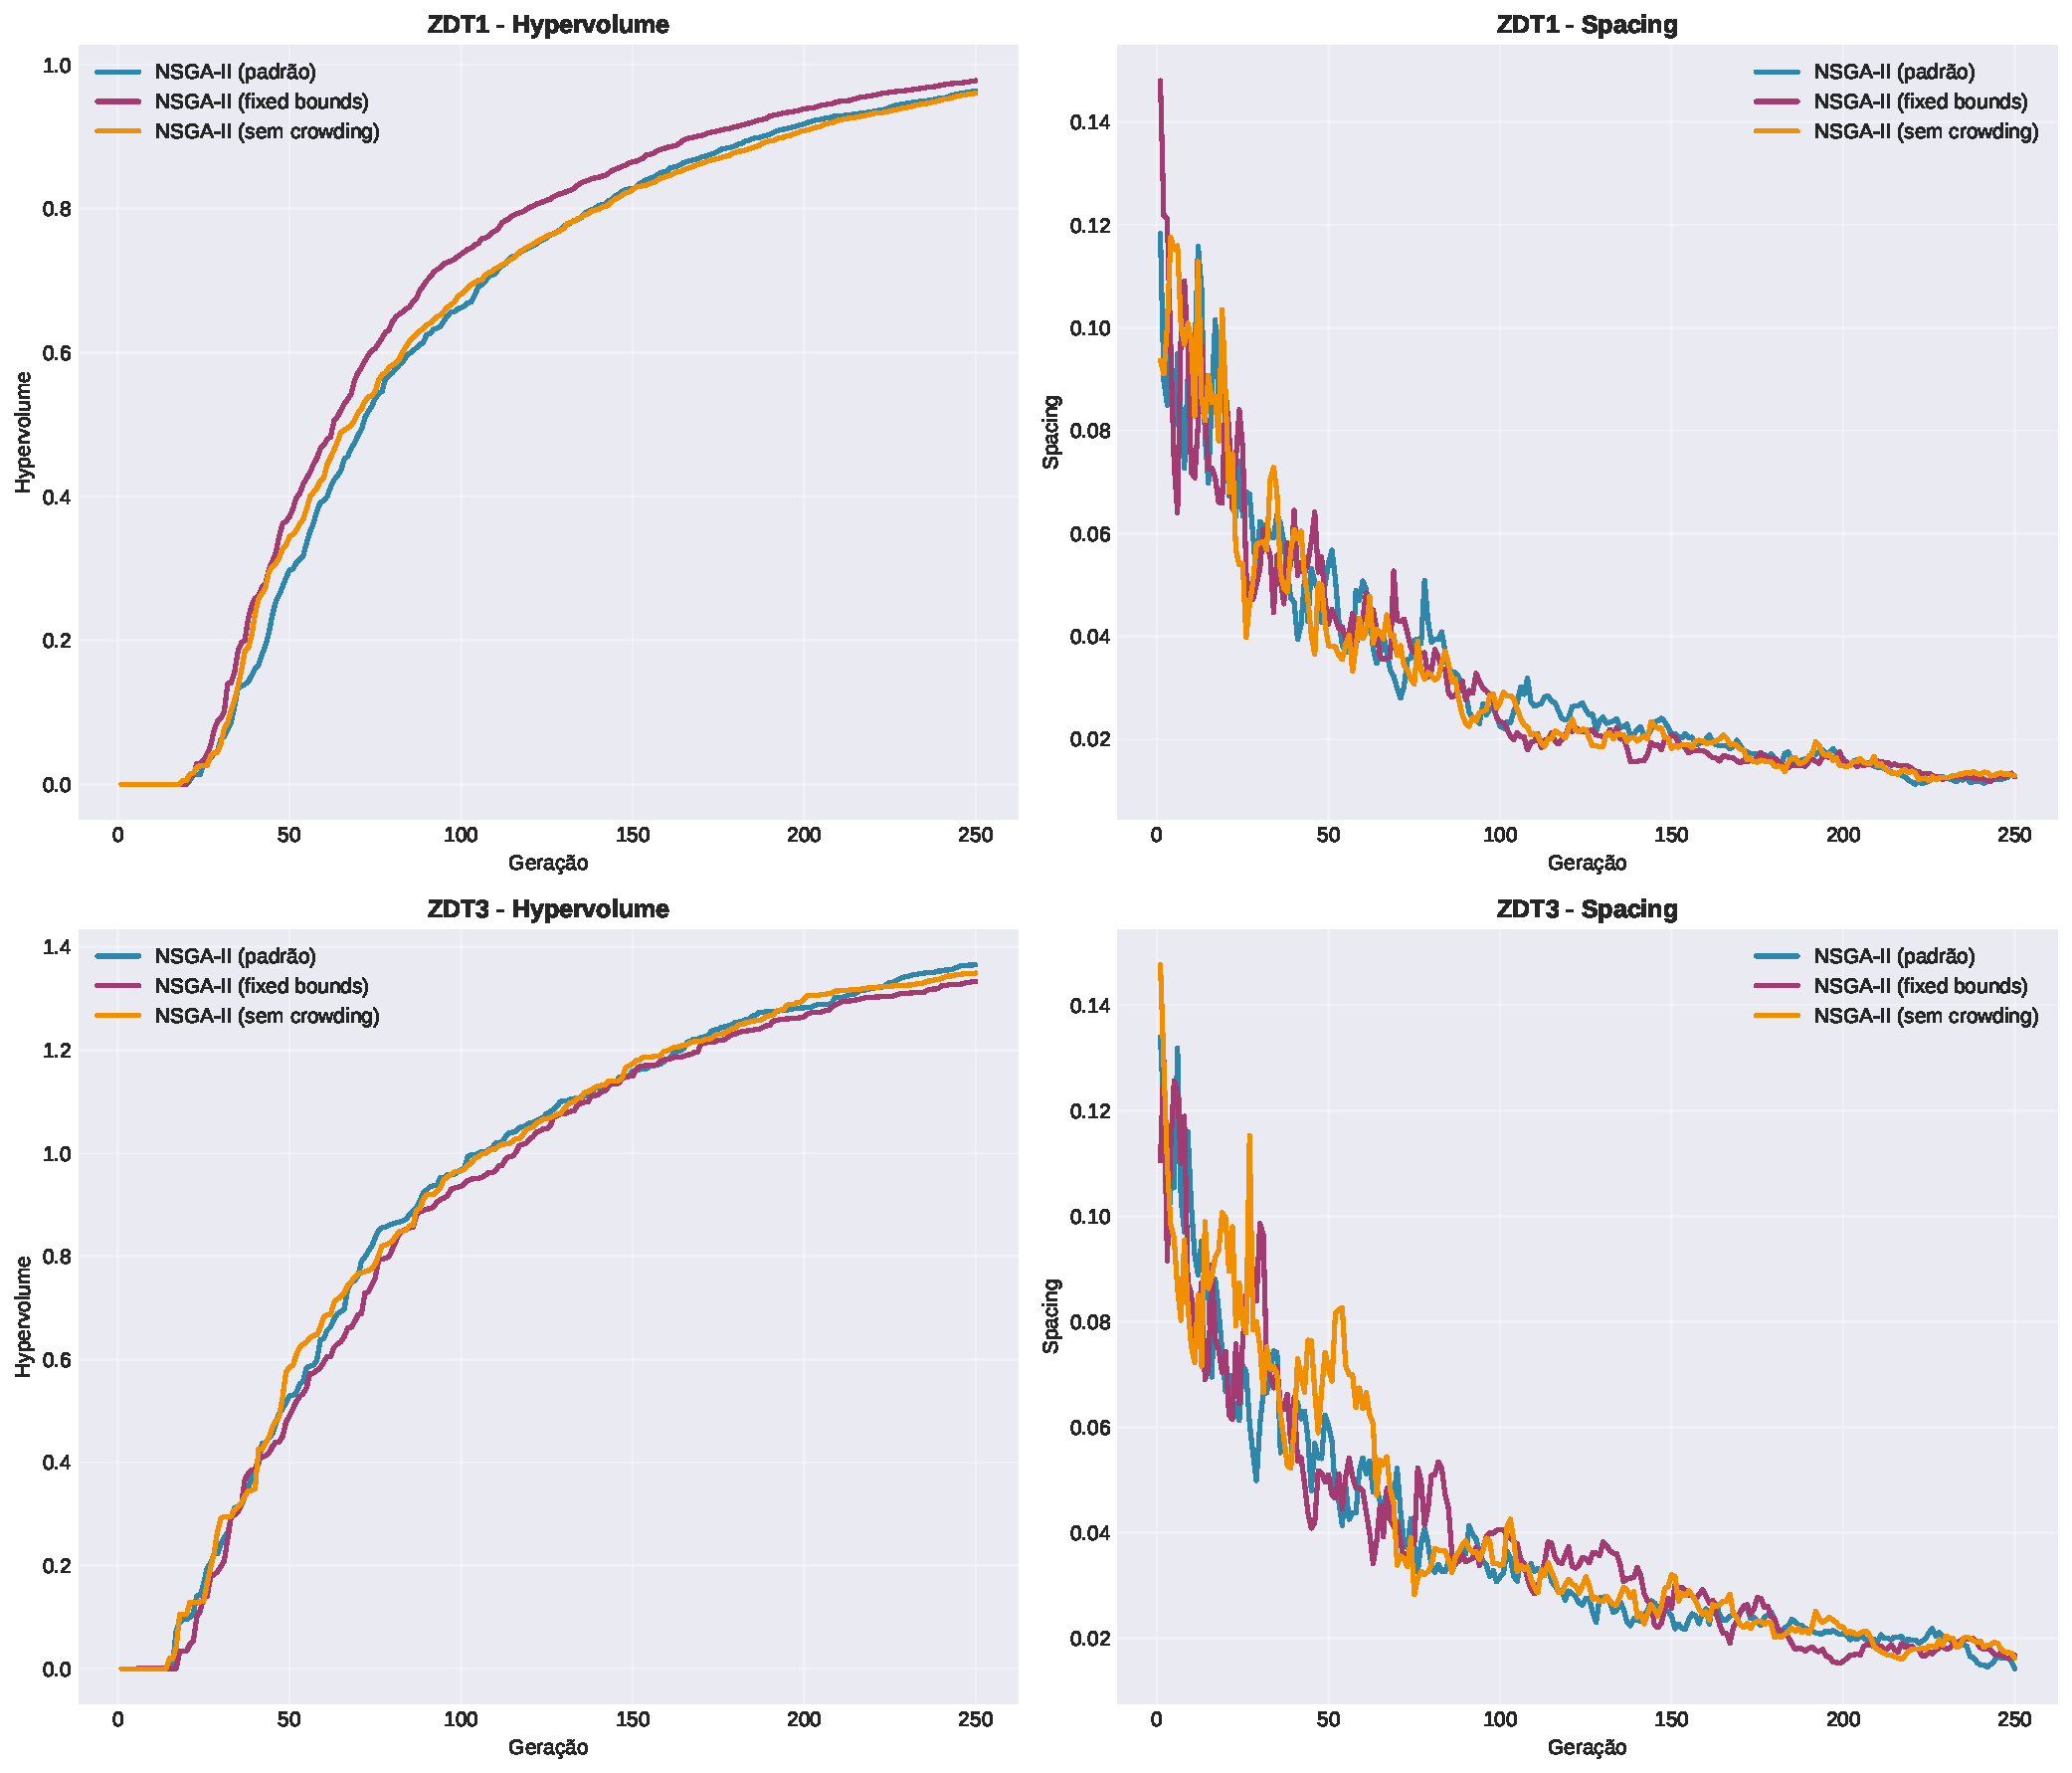
\includegraphics[width=\textwidth]{../plots/H_combined_metrics.pdf}
    \caption{Evolução normalizada de Hypervolume, Spacing (invertido) e Tamanho do Pareto para NSGA-II padrão. Normalização permite comparação direta das taxas de convergência. Hypervolume converge mais rapidamente que uniformidade de distribuição.}
    \label{fig:combined_metrics}
\end{figure}

\textbf{Insights de Sincronização}:
\begin{itemize}
    \item \textbf{Hypervolume lidera}: Atinge 90\% antes de Spacing e Tamanho do Pareto
    \item \textbf{Spacing atrasa}: Convergência 15-20 gerações posterior ao HV
    \item \textbf{Tamanho do Pareto oscila}: Não converge monotonicamente; reflete dinâmica de dominância
    \item \textbf{Implicação}: HV pode ser usado como critério de parada conservador
\end{itemize}

\subsection{Análise de Variabilidade Estocástica}

\subsubsection{Desvio Padrão Temporal}

Análise do envelope de desvio padrão (áreas sombreadas nas figuras):

\begin{itemize}
    \item \textbf{Fase inicial (0-20 gen.)}: Desvio alto ($\approx$10-15\% da média)
    \begin{itemize}
        \item Causa: Aleatoriedade da população inicial
        \item Comportamento esperado em MOEAs
    \end{itemize}
    
    \item \textbf{Fase intermediária (20-60 gen.)}: Redução progressiva para 3-5\%
    \begin{itemize}
        \item Convergência dos operadores genéticos
        \item Estabilização da estrutura populacional
    \end{itemize}
    
    \item \textbf{Fase final (60-250 gen.)}: Desvio mínimo ($<$2\%)
    \begin{itemize}
        \item Alta reprodutibilidade
        \item Convergência bem-comportada
    \end{itemize}
\end{itemize}

\subsubsection{Coeficiente de Variação}

Tabela~\ref{tab:cv_analysis} apresenta coeficientes de variação (CV = desvio/média) na geração 250.

\begin{table}[H]
\centering
\caption{Coeficiente de Variação (\%) na Geração Final}
\label{tab:cv_analysis}
\begin{tabular}{@{}lcccc@{}}
\toprule
\textbf{Algoritmo} & \textbf{HV (ZDT1)} & \textbf{HV (ZDT3)} & \textbf{Spacing (ZDT1)} & \textbf{Spacing (ZDT3)} \\
\midrule
NSGA-II (padrão) & 0.5\% & 0.7\% & 6.5\% & 5.4\% \\
NSGA-II (\textit{fixed bounds}) & 0.5\% & 0.7\% & 6.5\% & 4.3\% \\
NSGA-II (sem \textit{crowding}) & 1.5\% & 1.0\% & 5.3\% & 3.8\% \\
\textit{Random Search} & 4.2\% & N/A & 4.3\% & 4.1\% \\
\bottomrule
\end{tabular}
\end{table}

\textbf{Interpretação}:
\begin{itemize}
    \item HV altamente reproduzível (CV $<$ 1.5\%)
    \item Spacing mais sensível a estocasticidade (CV $\approx$ 5\%)
    \item Random Search tem maior variabilidade (esperado devido à natureza aleatória)
\end{itemize}

\subsection{Síntese da Análise de Convergência}

\subsubsection{Principais Descobertas}

\begin{enumerate}
    \item \textbf{Convergência Rápida do NSGA-II}:
    \begin{itemize}
        \item 90\% da performance final em apenas 18\% das gerações (45/250)
        \item Justifica uso de critérios de parada adaptativos baseados em HV
    \end{itemize}
    
    \item \textbf{Papel Crítico da \textit{Crowding Distance}}:
    \begin{itemize}
        \item Remoção causa degradação de 30\% no HV final
        \item Impacto maior em ZDT3 (33\%) devido à descontinuidade
        \item Essencial para manutenção de diversidade
    \end{itemize}
    
    \item \textbf{Impacto Limitado de \textit{Fixed Bounds}}:
    \begin{itemize}
        \item Diferença $<$ 1\% no HV final em ambos os problemas
        \item Ligeira vantagem em Spacing (15\% melhor em ZDT1)
        \item Normalização dinâmica suficientemente robusta
    \end{itemize}
    
    \item \textbf{Ineficácia do \textit{Random Search}}:
    \begin{itemize}
        \item HV estagnado em 10\% do NSGA-II
        \item Ausência de convergência observável
        \item Confirma necessidade de mecanismos evolutivos guiados
    \end{itemize}
\end{enumerate}

\subsubsection{Implicações Práticas}

\begin{itemize}
    \item \textbf{Eficiência computacional}: Executar $\approx$50 gerações pode ser suficiente para aplicações que toleram 5-10\% de subotimalidade
    
    \item \textbf{Monitoramento em tempo real}: HV serve como indicador confiável de convergência; Spacing complementa com informação sobre distribuição
    
    \item \textbf{Configuração robusta}: NSGA-II padrão demonstra performance consistente sem necessidade de ajuste de normalização
    
    \item \textbf{Problemas descontínuos}: Requerem mais gerações para uniformidade (Spacing), mas HV converge em taxa similar
\end{itemize}
